\documentclass{article}[18pt]
\ProvidesPackage{format}
%Page setup
\usepackage[utf8]{inputenc}
\usepackage[margin=0.7in]{geometry}
\usepackage{parselines} 
\usepackage[english]{babel}
\usepackage{fancyhdr}
\usepackage{titlesec}
\hyphenpenalty=10000

\pagestyle{fancy}
\fancyhf{}
\rhead{Sam Robbins}
\rfoot{Page \thepage}

%Characters
\usepackage{amsmath}
\usepackage{amssymb}
\usepackage{gensymb}
\newcommand{\R}{\mathbb{R}}

%Diagrams
\usepackage{pgfplots}
\usepackage{graphicx}
\usepackage{tabularx}
\usepackage{relsize}
\pgfplotsset{width=10cm,compat=1.9}
\usepackage{float}

%Length Setting
\titlespacing\section{0pt}{14pt plus 4pt minus 2pt}{0pt plus 2pt minus 2pt}
\newlength\tindent
\setlength{\tindent}{\parindent}
\setlength{\parindent}{0pt}
\renewcommand{\indent}{\hspace*{\tindent}}

%Programming Font
\usepackage{courier}
\usepackage{listings}
\usepackage{pxfonts}

%Lists
\usepackage{enumerate}
\usepackage{enumitem}

% Networks Macro
\usepackage{tikz}


% Commands for files converted using pandoc
\providecommand{\tightlist}{%
	\setlength{\itemsep}{0pt}\setlength{\parskip}{0pt}}
\usepackage{hyperref}

% Get nice commands for floor and ceil
\usepackage{mathtools}
\DeclarePairedDelimiter{\ceil}{\lceil}{\rceil}
\DeclarePairedDelimiter{\floor}{\lfloor}{\rfloor}

% Allow itemize to go up to 20 levels deep (just change the number if you need more you madman)
\usepackage{enumitem}
\setlistdepth{20}
\renewlist{itemize}{itemize}{20}

% initially, use dots for all levels
\setlist[itemize]{label=$\cdot$}

% customize the first 3 levels
\setlist[itemize,1]{label=\textbullet}
\setlist[itemize,2]{label=--}
\setlist[itemize,3]{label=*}

% Definition and Important Stuff
% Important stuff
\usepackage[framemethod=TikZ]{mdframed}

\newcounter{theo}[section]\setcounter{theo}{0}
\renewcommand{\thetheo}{\arabic{section}.\arabic{theo}}
\newenvironment{important}[1][]{%
	\refstepcounter{theo}%
	\ifstrempty{#1}%
	{\mdfsetup{%
			frametitle={%
				\tikz[baseline=(current bounding box.east),outer sep=0pt]
				\node[anchor=east,rectangle,fill=red!50]
				{\strut Important};}}
	}%
	{\mdfsetup{%
			frametitle={%
				\tikz[baseline=(current bounding box.east),outer sep=0pt]
				\node[anchor=east,rectangle,fill=red!50]
				{\strut Important:~#1};}}%
	}%
	\mdfsetup{innertopmargin=10pt,linecolor=red!50,%
		linewidth=2pt,topline=true,%
		frametitleaboveskip=\dimexpr-\ht\strutbox\relax
	}
	\begin{mdframed}[]\relax%
		\centering
		}{\end{mdframed}}



\newcounter{lem}[section]\setcounter{lem}{0}
\renewcommand{\thelem}{\arabic{section}.\arabic{lem}}
\newenvironment{defin}[1][]{%
	\refstepcounter{lem}%
	\ifstrempty{#1}%
	{\mdfsetup{%
			frametitle={%
				\tikz[baseline=(current bounding box.east),outer sep=0pt]
				\node[anchor=east,rectangle,fill=blue!20]
				{\strut Definition};}}
	}%
	{\mdfsetup{%
			frametitle={%
				\tikz[baseline=(current bounding box.east),outer sep=0pt]
				\node[anchor=east,rectangle,fill=blue!20]
				{\strut Definition:~#1};}}%
	}%
	\mdfsetup{innertopmargin=10pt,linecolor=blue!20,%
		linewidth=2pt,topline=true,%
		frametitleaboveskip=\dimexpr-\ht\strutbox\relax
	}
	\begin{mdframed}[]\relax%
		\centering
		}{\end{mdframed}}
\lhead{CT - ECC}


\begin{document}
\begin{center}
\underline{\huge Decoder error probability}
\end{center}
\section{Error v failure}
\subsection{Probabilistic channels}
Recall the source-channel-reciever diagram\\
Channels are probabilistic in nature. Errors due to thermal noise, faults, damage...\\
Impossible to predict how many errors will occur
\subsection{Decoder error and failure}
If more than t errors occur, two situations could happen
\begin{itemize}
	\item The decoder cannot find any codeword at a distance $\leqslant$ t from the received vector: Decoder \textbf{failure}
	\item The decoder finds another (wrong) codeword at distance $\leqslant$ t from the received vector: Decoder \textbf{error}
\end{itemize}
Failure: Ask for retransmission. No big deal\\
Error: the decoder is totally oblivious. Much more problematic.\\
No failures when using hamming codes - hamming codes are optimal so all sequences will correspond to a codeword.
\subsection{Example of decoder error and failure}
Consider the code with the following parity-check matrix:
$$H = \left( \begin{array} { l l l l l } { 0 } & { 0 } & { 0 } & { 1 } & { 1 } \\ { 0 } & { 1 } & { 1 } & { 0 } & { 0 } \\ { 1 } & { 0 } & { 1 } & { 0 } & { 1 } \end{array} \right)$$
This is a (5,2,3)-code. It's codewords are:
$$\{ ( 0,0,0,0,0 ) , ( 0,1,1,1,1 ) , ( 1,1,1,0,0 ) , ( 1,0,0,1,1 ) \}$$
Suppose we send the all zero codeword C=(0,0,0,0,0)
\begin{itemize}
	\item If the vector v=(0,1,0,1,0) is received: failure
	\item If the vector v=(1,1,0,0,0) is received: error
\end{itemize}
\section{Decoder error probability}
In general, the decoder error probability (DEP) depends on:
\begin{itemize}
	\item The channel
	\item The code we use
	\item The transmitted codeword
\end{itemize}
For a given channel and a given code, it can be determined
\subsection{Binary symmetric channel}
Instead of trying to figure out exactly how the errors occur, we will simplify the channel model\\
\\
Binary symmetric channel (BSC) with crossover probability p:
\begin{center}
	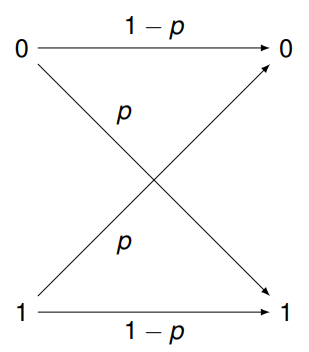
\includegraphics[scale=0.7]{bsc1}
\end{center}
\subsection{How many errors?}
Let E be the number of errors under a BSC, if n bits are transmitted. We have:
$$P ( E = w ) = \left( \begin{array} { c } { n } \\ { w } \end{array} \right) p ^ { w } ( 1 - p ) ^ { n - w }$$
If we use a code with error correction capability t, the probability of not being able to correct the errors is:
$$\begin{aligned} P ( E > t ) & = 1 - P ( E \leq t ) \\ & = 1 - \sum _ { w = 0 } ^ { t } \left( \begin{array} { l } { n } \\ { w } \end{array} \right) p ^ { w } ( 1 - p ) ^ { n - w } \end{aligned}$$
\subsection{DEP over the BSC}
\textbf{Theorem:} Let $A_i(c)$ be the number of codewords at distance i from the transmitted codeword \textbf{c}, then the DEP over a BSC with crossover probability p is
$$D E P = \sum _ { w = t + 1 } ^ { n } p ^ { w } ( 1 - p ) ^ { n - w } \sum _ { i = d _ { m i n } } ^ { n } A _ { i } ( \mathbf { c } ) \sum _ { s = 0 } ^ { t } \left( \begin{array} { c } { i } \\ { \frac { w - s + i } { 2 } } \end{array} \right) \left( \begin{array} { c } { n - i } \\ { \frac { w + s - i } { 2 } } \end{array} \right)$$
Where
$$\left( \begin{array} { l } { a } \\ { b } \end{array} \right) = \left\{ \begin{array} { l l } { \frac { a ! } { b ! ( a - b ) ! } } & { \text { if } 0 \leq b \leq a \text { are integers } } \\ { 0 } & { \text { otherwise } } \end{array} \right.$$
\subsection{Distance distribution of Hamming codes}
For any linear code, $A_i(C)$ does not depend on c\\
For the $\left( n = 2 ^ { r } - 1 , k = 2 ^ { r } - r - 1,3 \right)$-Hamming code
$$A _ { i } = 2 ^ { - r } \left( \begin{array} { c } { 2 ^ { r } - 1 } \\ { i } \end{array} \right) + \left( 1 - 2 ^ { - r } \right) \sum _ { j = 0 } ^ { i } ( - 1 ) ^ { j } \left( \begin{array} { c } { 2 ^ { r - 1 } } \\ { j } \end{array} \right) \left( \begin{array} { c } { 2 ^ { r - 1 } - 1 } \\ { i - j } \end{array} \right)$$
\subsection{DEP of hamming codes}
For Hamming codes, you can apply the last two (long) equations.\\
\\
Alternatively, realise that there are \textbf{no failures} when using hamming codes. This, for a BSC channel with crossover probability p
$$D E P _ { \text { Hamming } } = P ( E > 1 ) = 1 - ( 1 - p ) ^ { n } - n p ( 1 - p ) ^ { n - 1 }$$
\end{document}